\subsection{Esercizio 1}
\begin{figure}[H]
\centering
\begin{subfigure}[b]{0.4\textwidth}
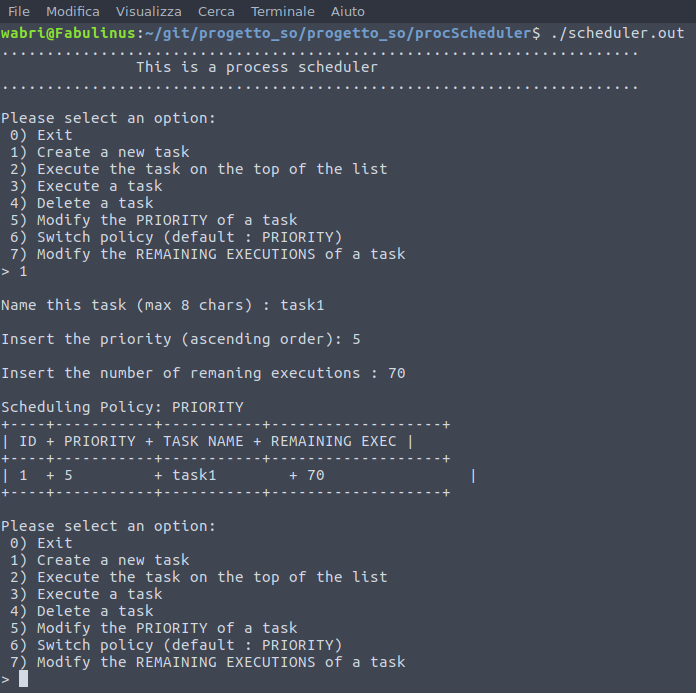
\includegraphics[width=\textwidth]{progetto_so/procScheduler/screenshot/1_new_task_without_error}
\caption{inserimento}
\end{subfigure}
\begin{subfigure}[b]{0.4\textwidth}
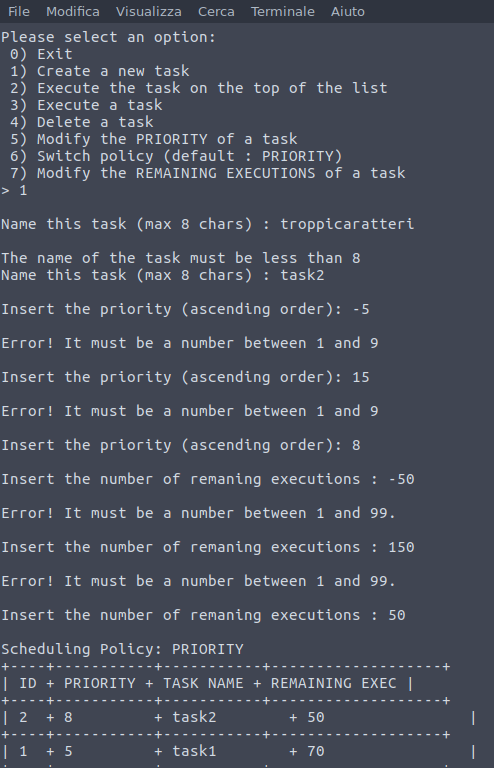
\includegraphics[width=\textwidth]{progetto_so/procScheduler/screenshot/2_new_task_with_error}
\caption{inseriemento con errore}
\end{subfigure}
\begin{subfigure}[b]{0.4\textwidth}
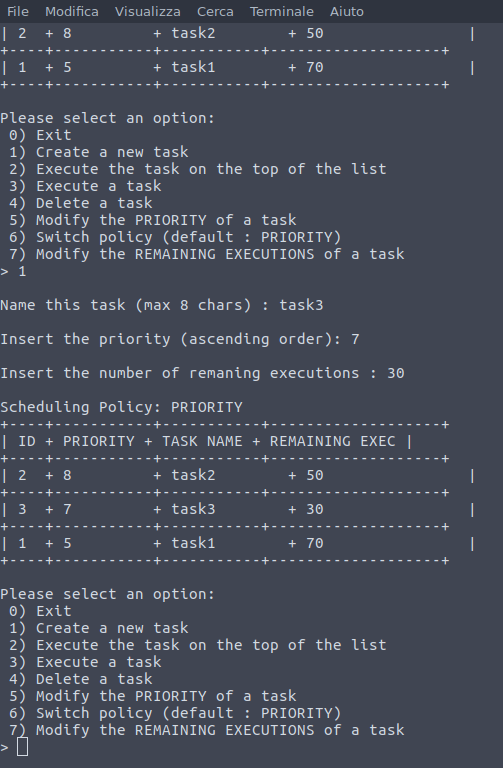
\includegraphics[width=\textwidth]{progetto_so/procScheduler/screenshot/3_new_task_sorting_policy_work}
\caption{inserimento e ordinamento}
\end{subfigure}
\caption{Creazione di un nuovo task}
\end{figure}

\begin{figure}
\centering
\begin{subfigure}[b]{0.4\textwidth}
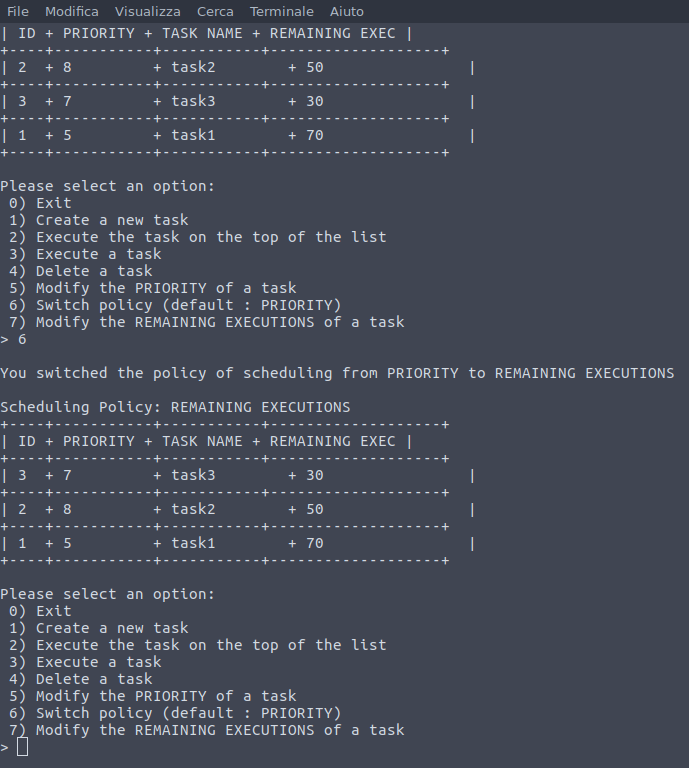
\includegraphics[width=\textwidth]{progetto_so/procScheduler/screenshot/4_change_policy_of_scheduler}
\caption{switch della politica di scheduling}
\end{subfigure}
\begin{subfigure}[b]{0.4\textwidth}
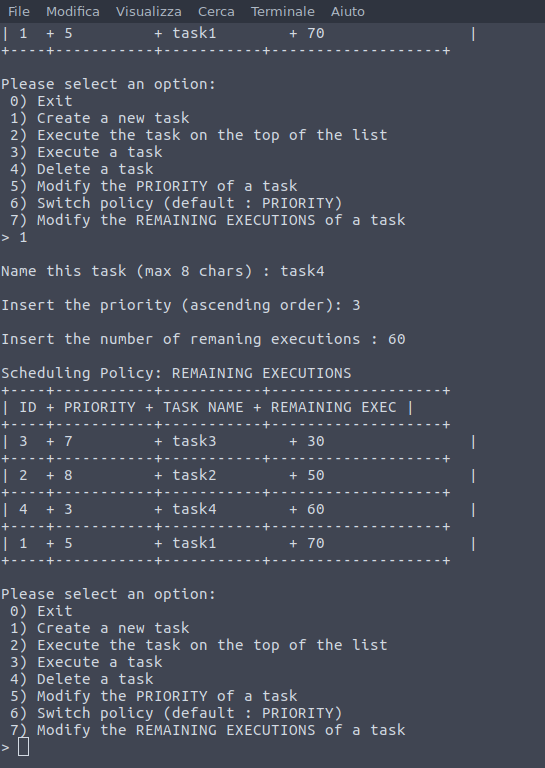
\includegraphics[width=\textwidth]{progetto_so/procScheduler/screenshot/5_new_task_added_to_test_policy_work}
\caption{inserimento e ordinamento}
\end{subfigure}
\begin{subfigure}[b]{0.4\textwidth}
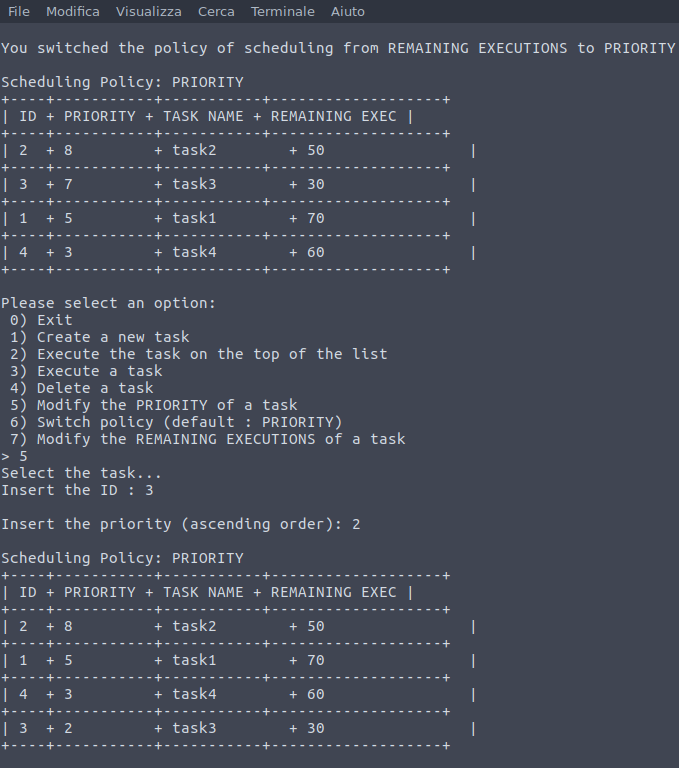
\includegraphics[width=\textwidth]{progetto_so/procScheduler/screenshot/6_switch_policy_and_modify_priority_of_a_task}
\caption{switch della policy e modifica della priori\'a}
\end{subfigure}
\caption{Mantenimento dell'ordinamento della lista dei task e modifica ai parametri}
\end{figure}

\begin{figure}
\centering
\begin{subfigure}[b]{0.4\textwidth}
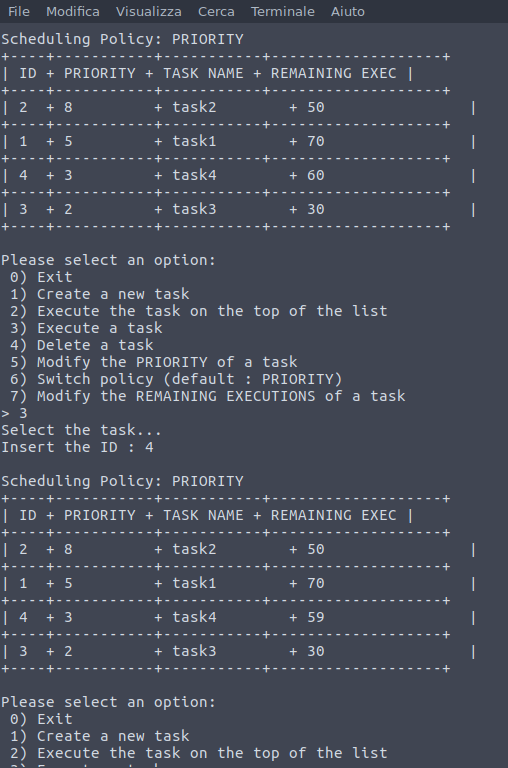
\includegraphics[width=\textwidth]{progetto_so/procScheduler/screenshot/7_single_execution_of_a_task}
\caption{singola esecuzione di un task}
\end{subfigure}
\begin{subfigure}[b]{0.4\textwidth}
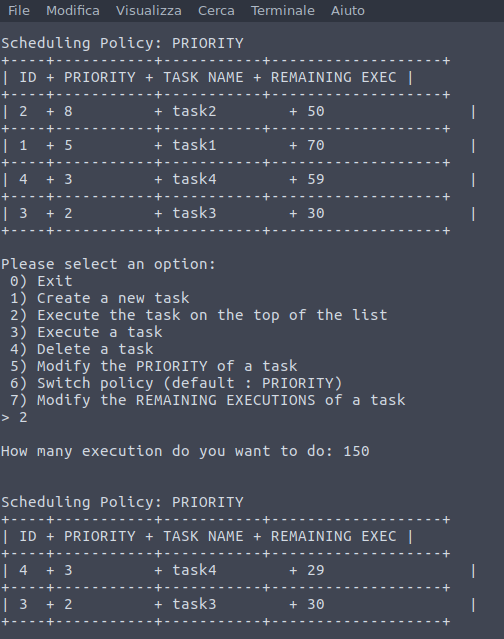
\includegraphics[width=\textwidth]{progetto_so/procScheduler/screenshot/8_150_executions_of_head_tasks}
\caption{150 esecuzioni dei task in testa}
\end{subfigure}
\begin{subfigure}[b]{0.4\textwidth}
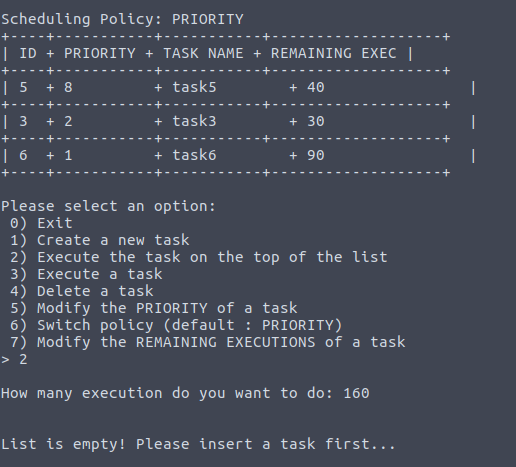
\includegraphics[width=\textwidth]{progetto_so/procScheduler/screenshot/10_execution_of_all_tasks}
\caption{esecuzione di tutti i task}
\end{subfigure}
\caption{Esecuzioni varie dei task}
\end{figure}

\begin{figure}
\centering
\begin{subfigure}[b]{0.4\textwidth}
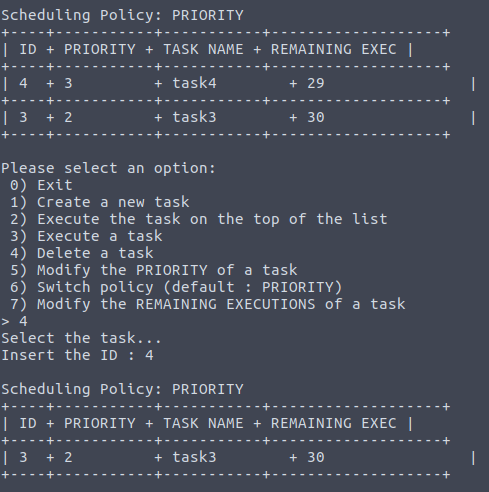
\includegraphics[width=\textwidth]{progetto_so/procScheduler/screenshot/9_deletion_of_a_task}
\caption{eliminazione di tutti i task}
\end{subfigure}
\begin{subfigure}[b]{0.4\textwidth}
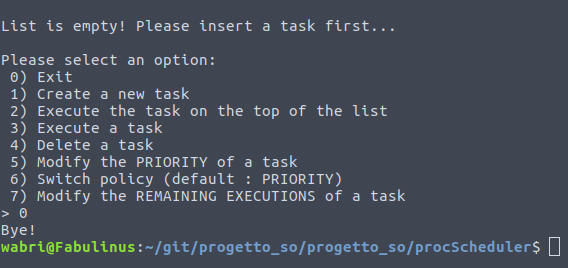
\includegraphics[width=\textwidth]{progetto_so/procScheduler/screenshot/11_exit}
\caption{uscita dal programma}
\end{subfigure}
\caption{Eliminazione dei task ed uscita dal programma}
\end{figure}

\subsubsection{Stress Test}

\begin{figure}[H]
\centering
\begin{subfigure}[b]{0.4\textwidth}
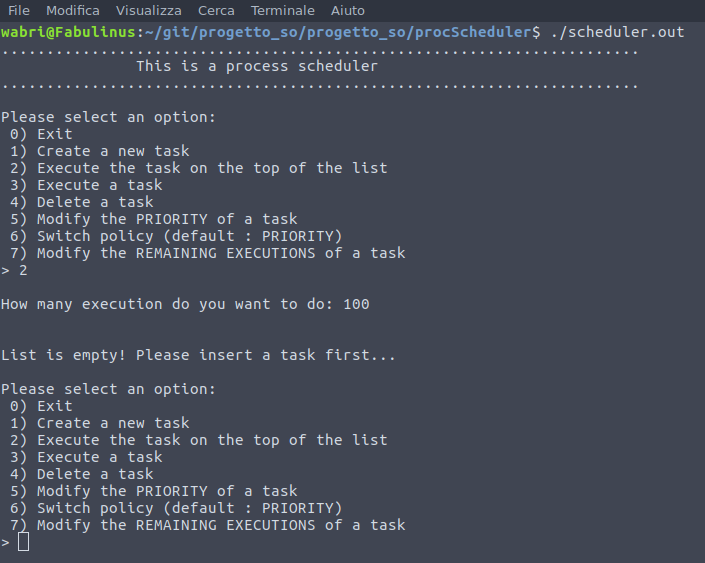
\includegraphics[width=\textwidth]{progetto_so/procScheduler/screenshot/12_stress_test_execute_when_no_tasks_are_in_the_task_list}
\caption{esecuzione a lista vuota}
\end{subfigure}
\begin{subfigure}[b]{0.4\textwidth}
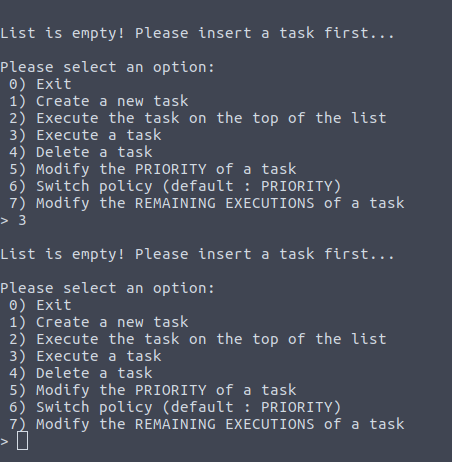
\includegraphics[width=\textwidth]{progetto_so/procScheduler/screenshot/13_stress_test_execute_with_id_when_no_tasks_are_in_the_task_list}
\caption{esecuzione per ID a lista vuota}
\end{subfigure}
\begin{subfigure}[b]{0.4\textwidth}
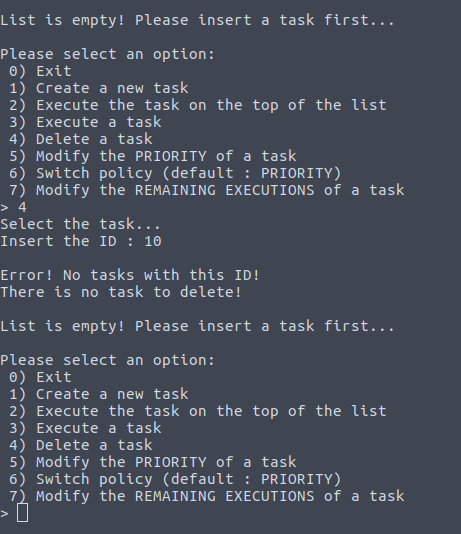
\includegraphics[width=\textwidth]{progetto_so/procScheduler/screenshot/14_stress_test_delete_with_id_when_no_tasks_are_in_the_task_list}
\caption{eliminazione per ID a lista vuota}
\end{subfigure}
\caption{Esecuzioni a lista vuota}
\end{figure}

\begin{figure}
\centering
\begin{subfigure}[b]{0.6\textwidth}
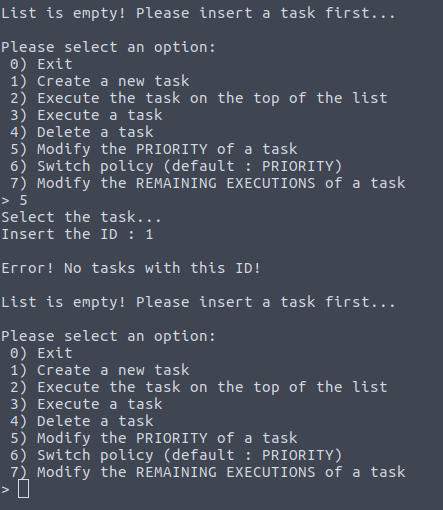
\includegraphics[width=\textwidth]{progetto_so/procScheduler/screenshot/15_stress_test_request_priority_edit_when_no_tasks_are_in_the_list}
\caption{modifica della priorit\'a a lista vuota}
\end{subfigure}
\begin{subfigure}[b]{0.6\textwidth}
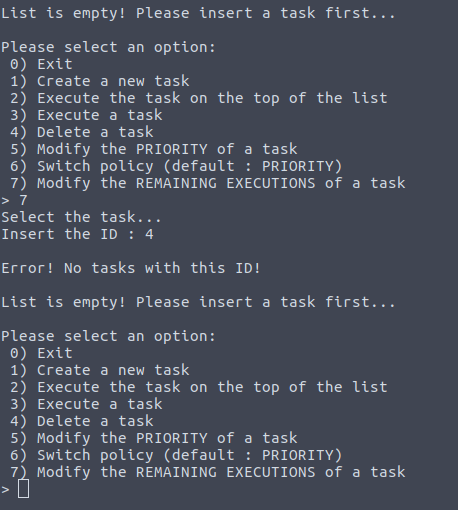
\includegraphics[width=\textwidth]{progetto_so/procScheduler/screenshot/16_stress_test_request_remaining_execution_edit_when_no_tasks_are_in_the_list}
\caption{modifica del n.esec. a lista vuota}
\end{subfigure}
\caption{Modifiche a lista vuota}
\end{figure}

\subsection{Esercizio 2}
\subsection{Esercizio 3}

\begin{itemize}
\item lancio del client con pid 6864 \\
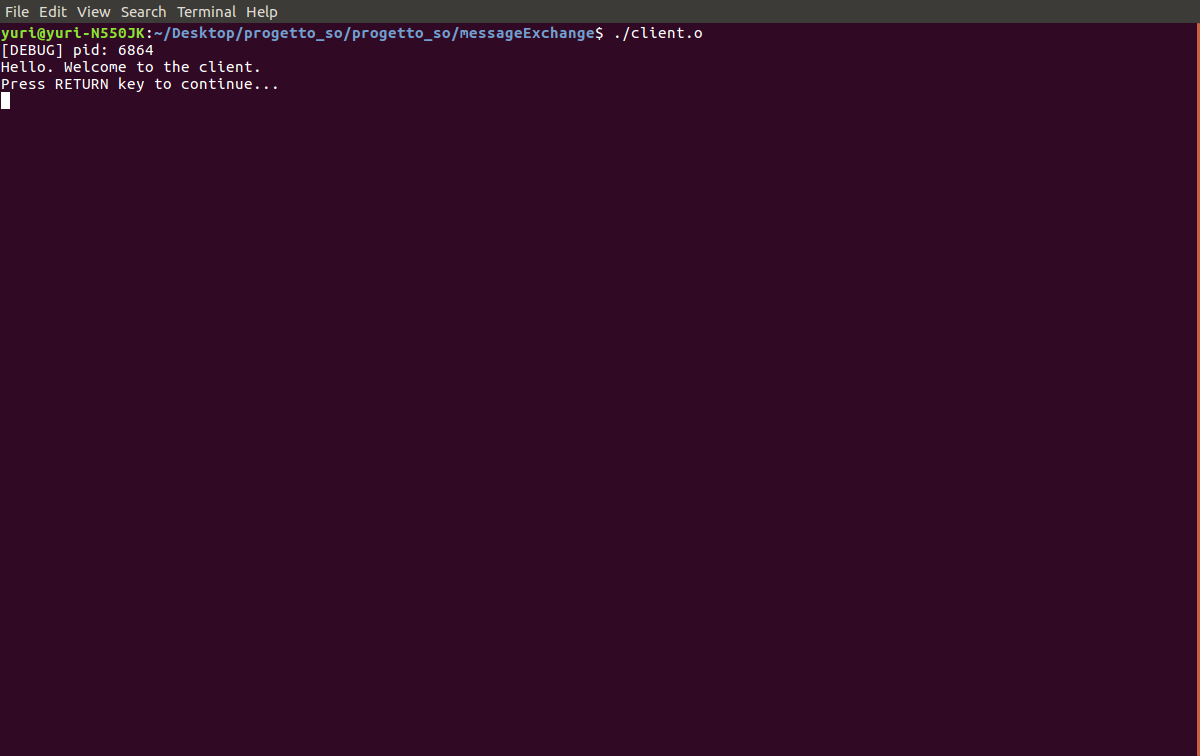
\includegraphics[scale=0.3]{screenmsg/1_client_6864}

\item comparsa del menu \\
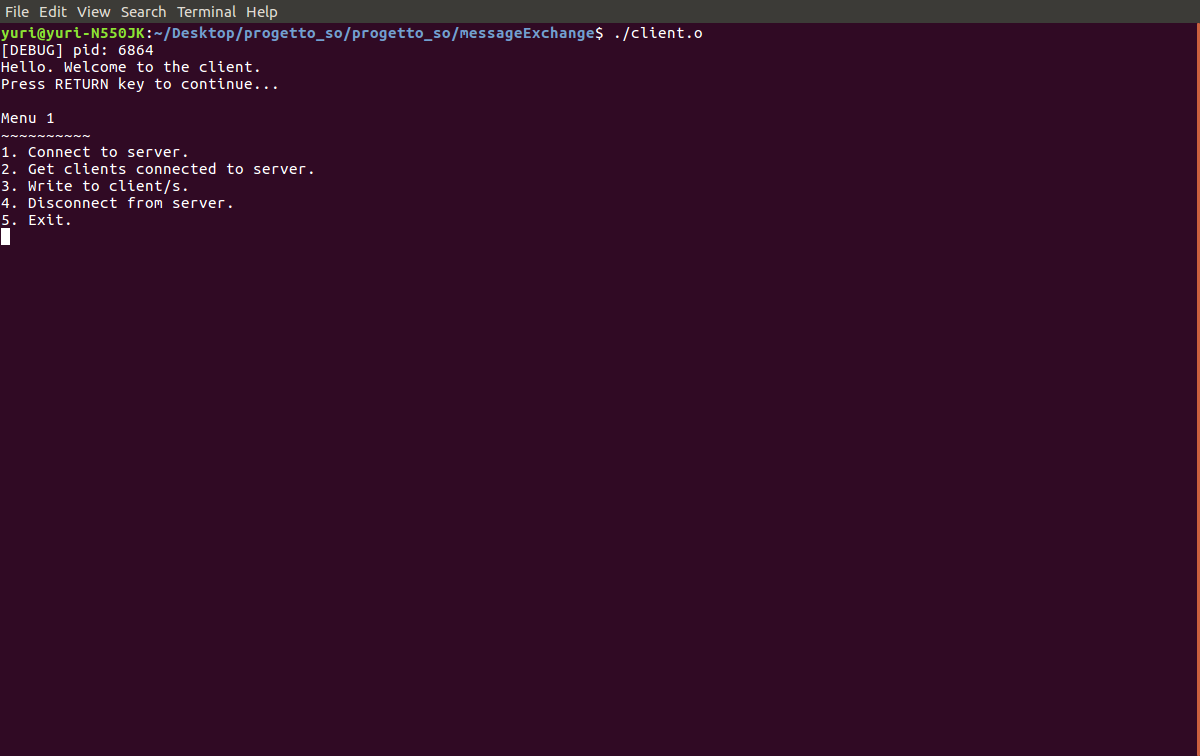
\includegraphics[scale=0.3]{screenmsg/2_client_6864}
\newpage
\item connessione del client 6864 al server \\
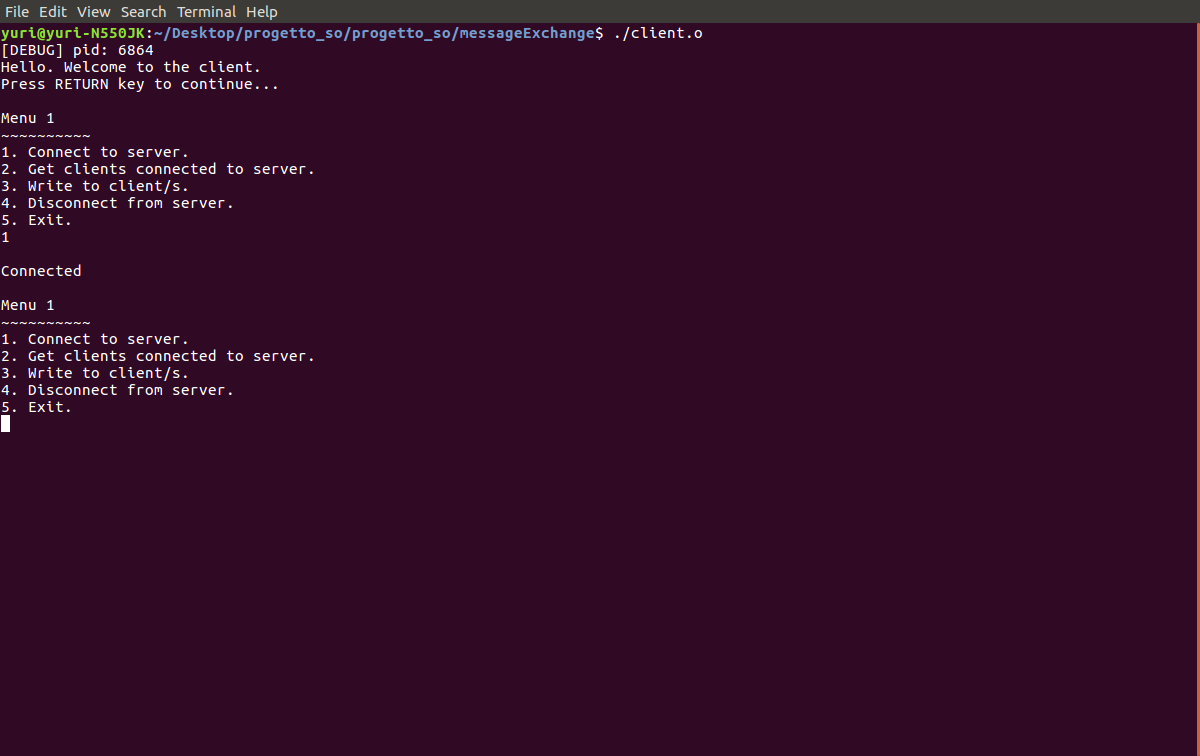
\includegraphics[scale=0.4]{screenmsg/3_client_6864}

\item connessione del client 6932 al server \\
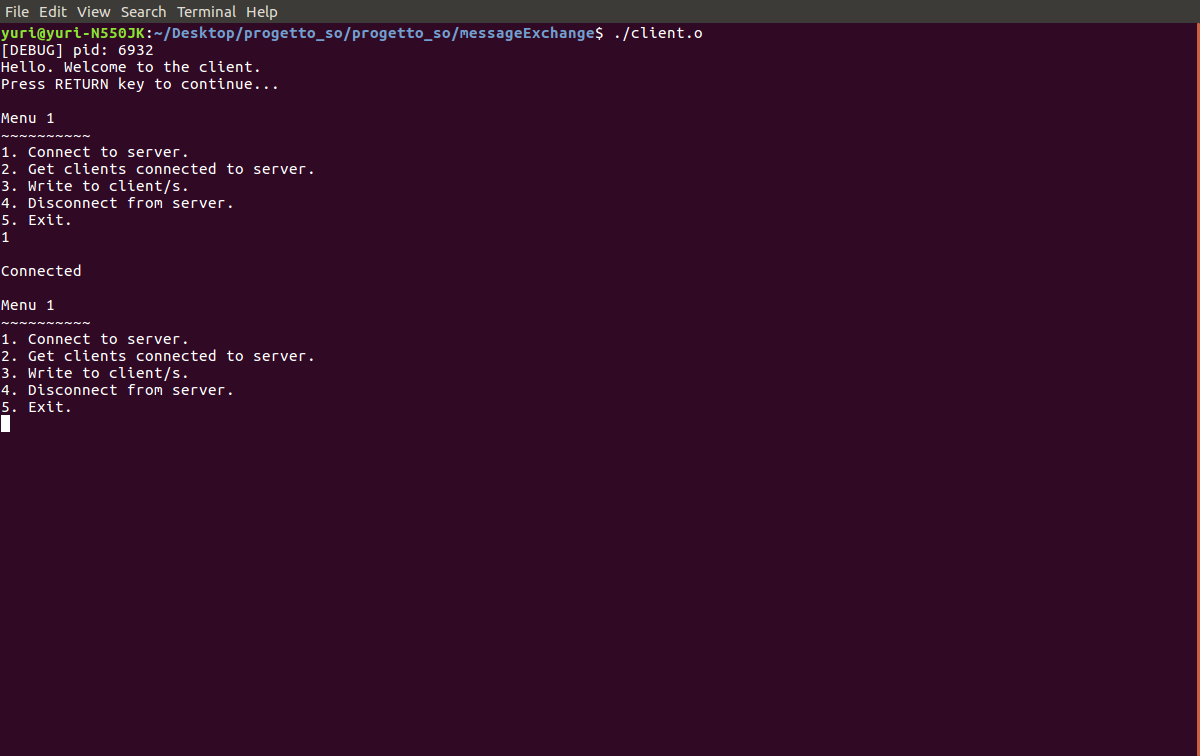
\includegraphics[scale=0.4]{screenmsg/4_client_6932}


\end{itemize}


\begin{figure}[H]
\centering
\begin{subfigure}[b]{0.7\textwidth}
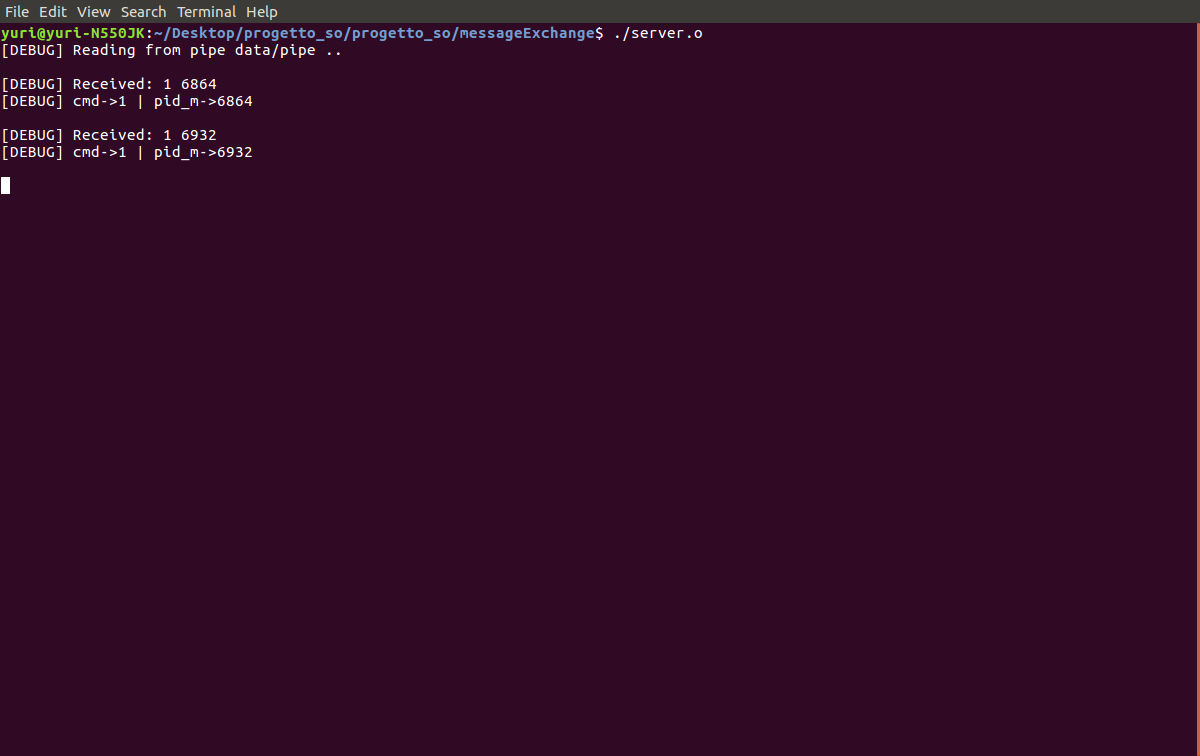
\includegraphics[width=\textwidth]{screenmsg/5_server}
\caption{Connessioni dei client 6864 e 6932 lato server}
\end{subfigure}
\begin{subfigure}[b]{0.7\textwidth}
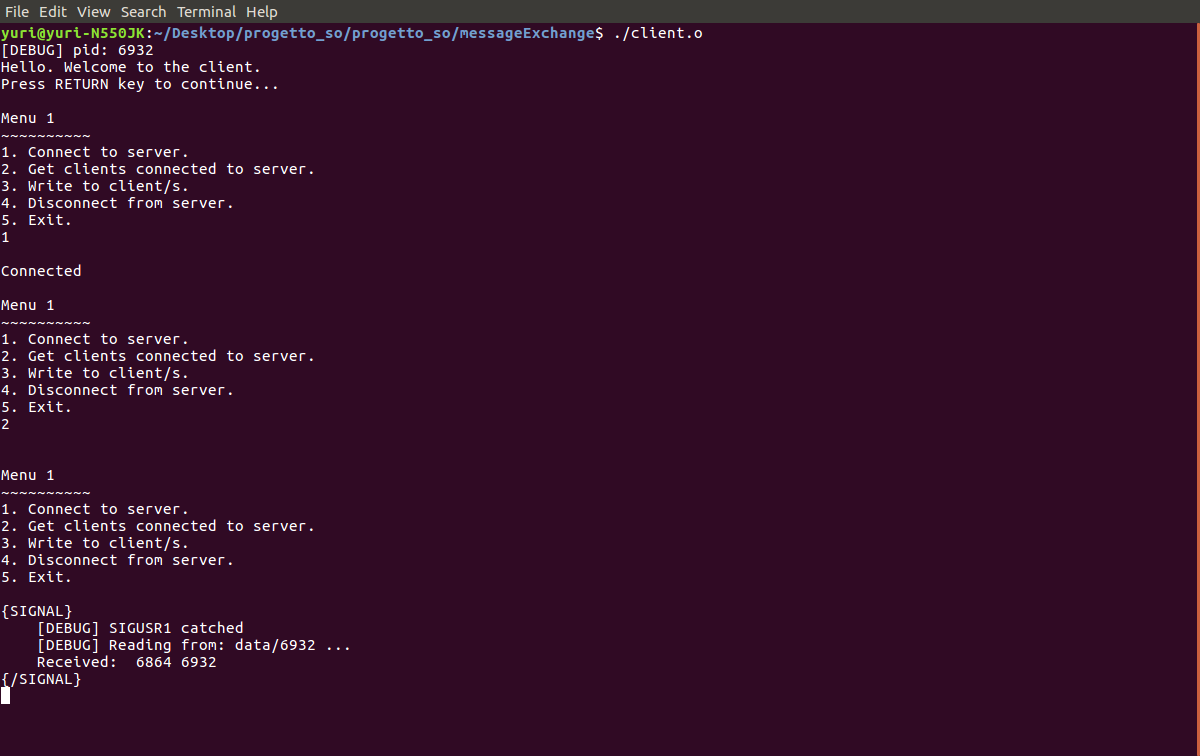
\includegraphics[width=\textwidth]{screenmsg/6_client_6932}
\caption{Richiesta da parte di 6932 dei client connessi}
\end{subfigure}
\begin{subfigure}[b]{0.7\textwidth}
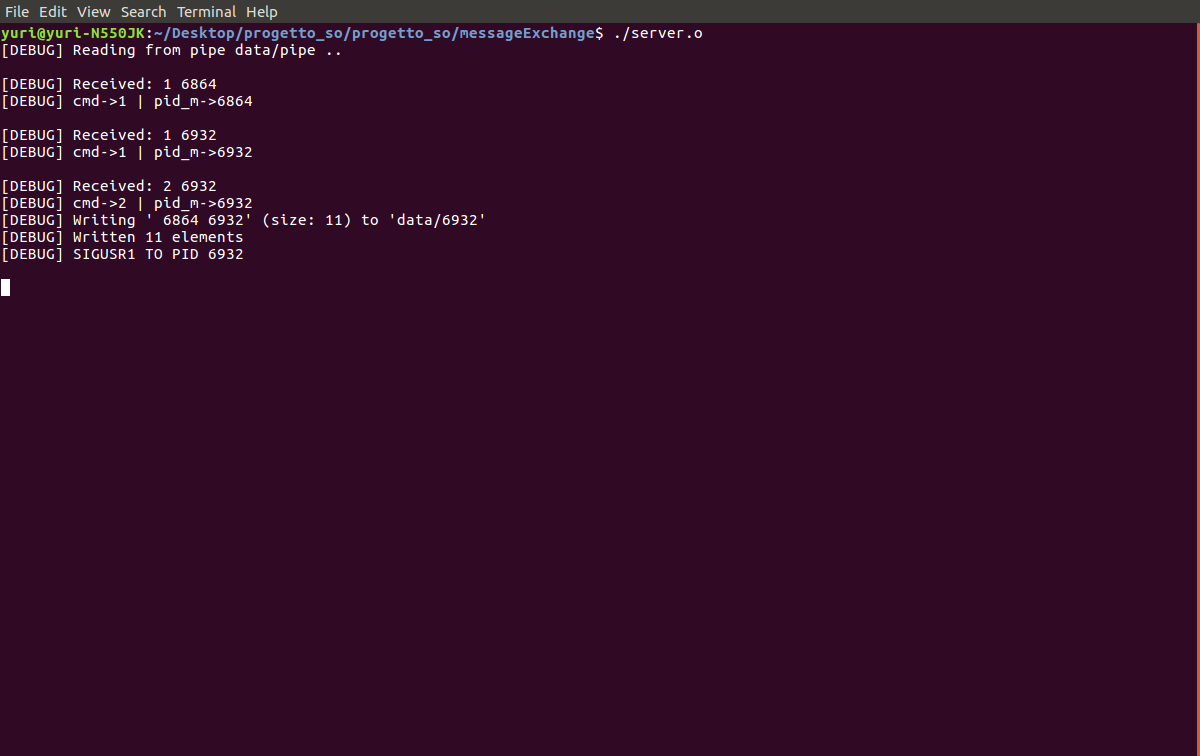
\includegraphics[width=\textwidth]{screenmsg/7_server}
\caption{Risposta del server a 6932}
\end{subfigure}
\caption{Connessioni e richiesta dei client connessi}
\end{figure}

\begin{figure}
\centering
\begin{subfigure}[b]{0.7\textwidth}
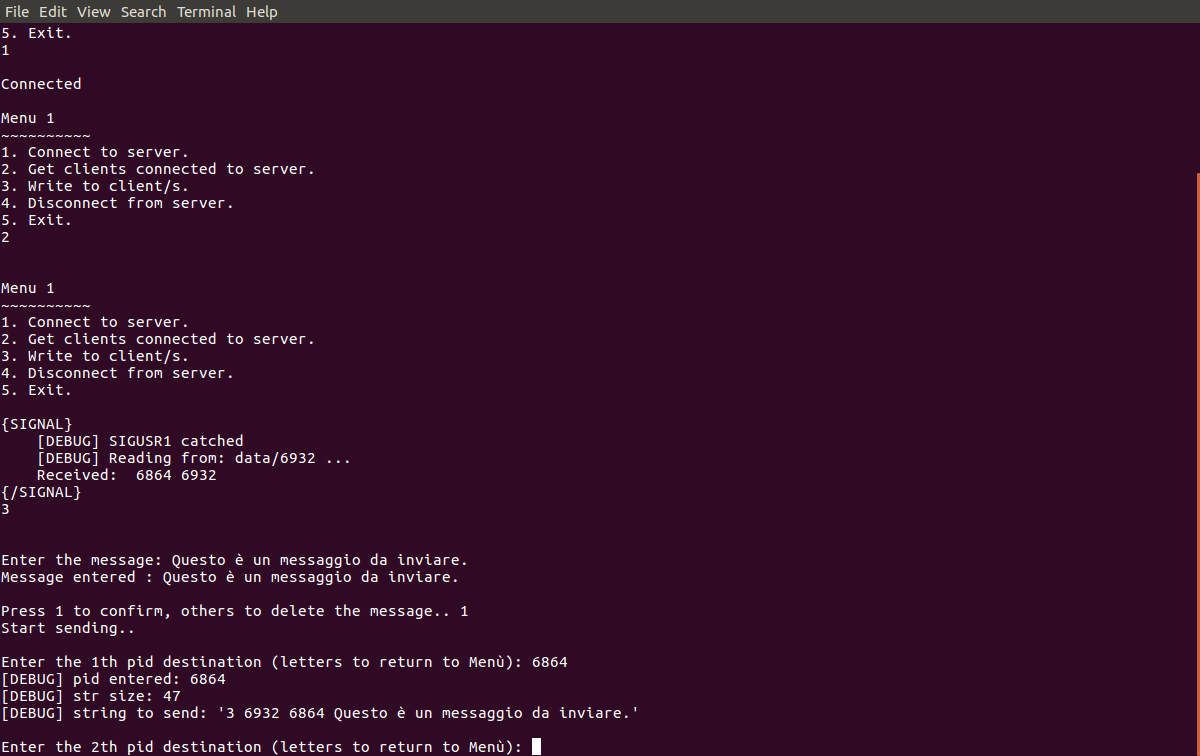
\includegraphics[width=\textwidth]{screenmsg/8_client_6932}
\caption{6932 invia un messaggio a 6864}
\end{subfigure}
\begin{subfigure}[b]{0.7\textwidth}
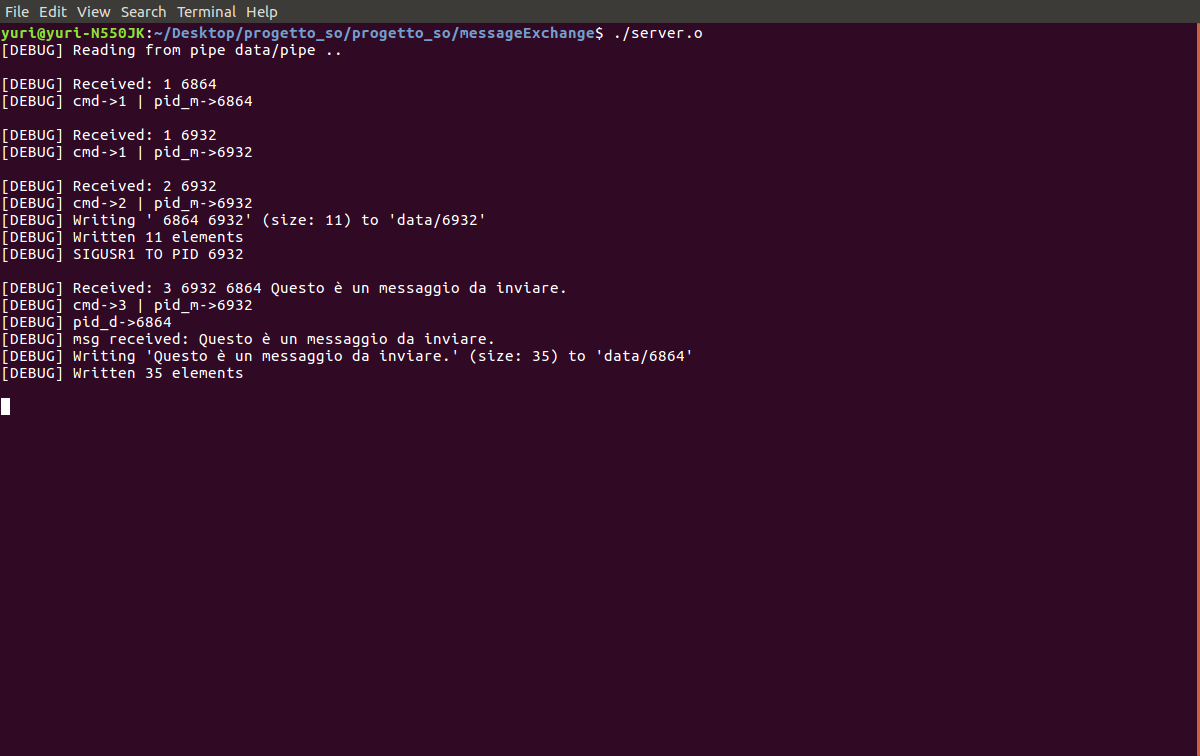
\includegraphics[width=\textwidth]{screenmsg/9_server}
\caption{Risposta del server alla richiesta di 6932}
\end{subfigure}
\begin{subfigure}[b]{0.7\textwidth}
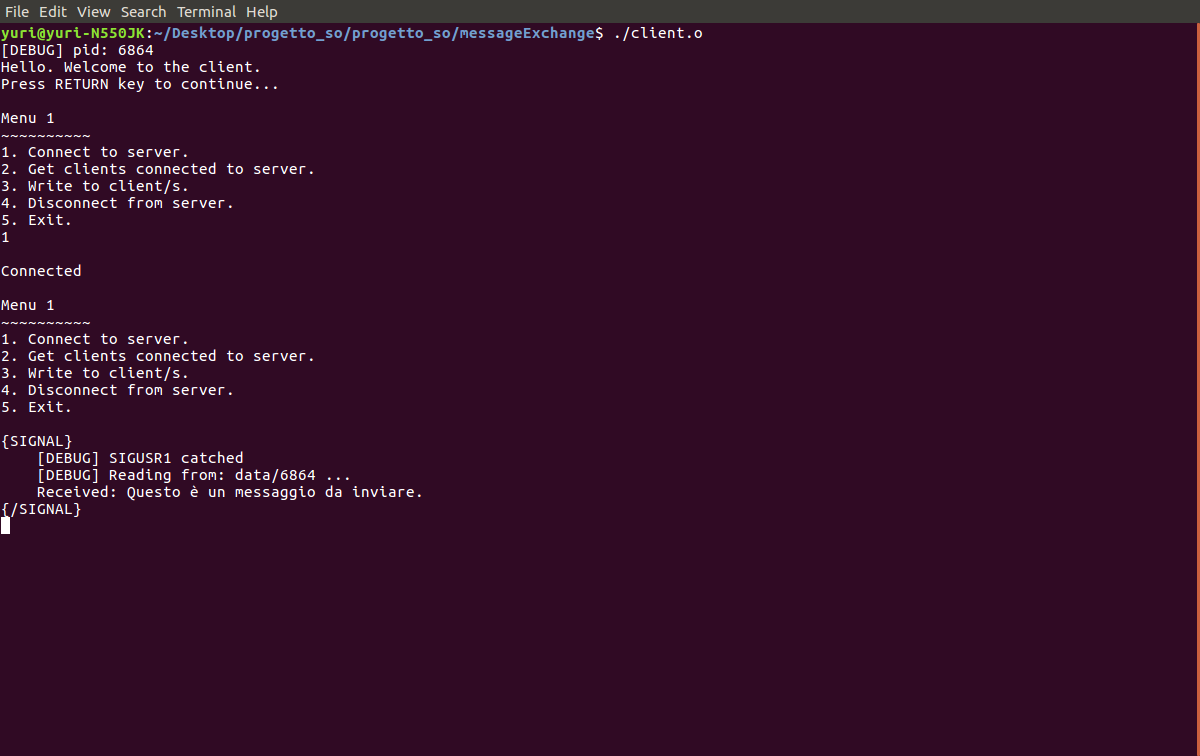
\includegraphics[width=\textwidth]{screenmsg/10_client_6864}
\caption{Ricezione del messaggio da parte di 6864}
\end{subfigure}
\caption{Message passing}
\end{figure}

\begin{figure}
\centering
\begin{subfigure}[b]{0.8\textwidth}
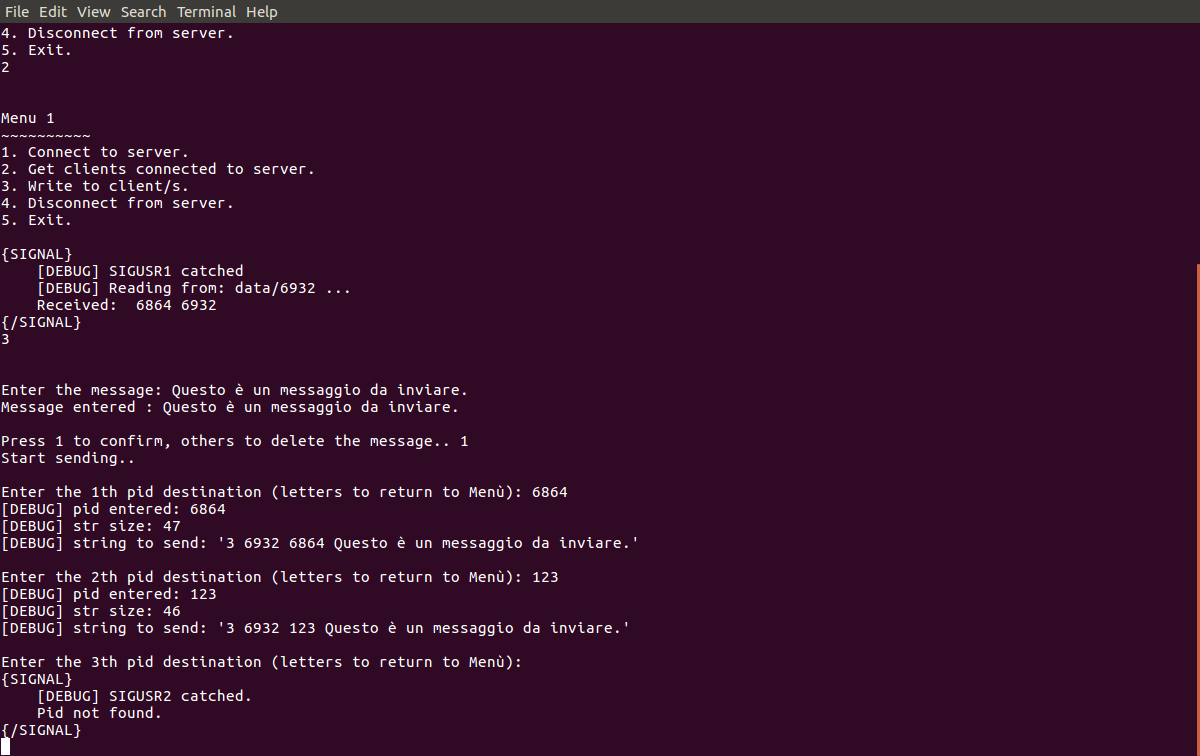
\includegraphics[width=\textwidth]{screenmsg/11_client_6932}
\caption{Gestione dell'errore nell'invio di un messaggio ad un client inesistente}
\end{subfigure}
\begin{subfigure}[b]{0.8\textwidth}
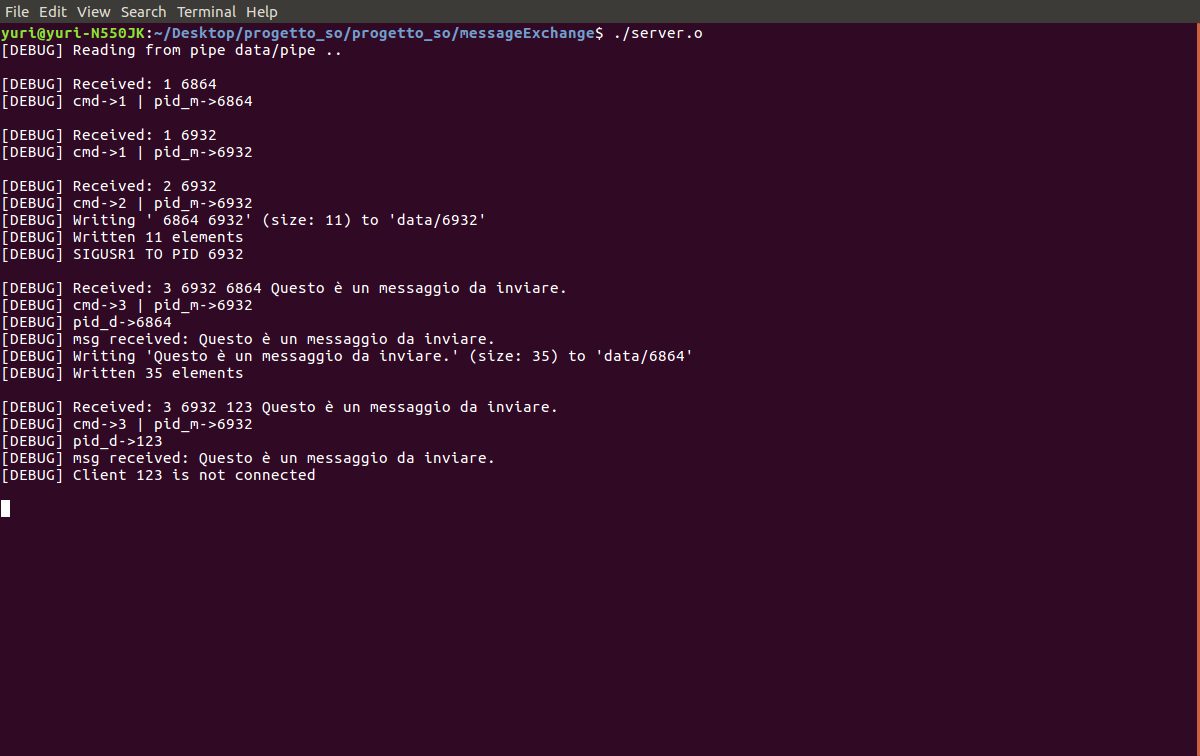
\includegraphics[width=\textwidth]{screenmsg/12_server}
\caption{Gestione dell'errore nell'invio di un messaggio ad un client inesistente lato server}
\end{subfigure}
\caption{Errori}
\end{figure}

\begin{figure}
\centering
\begin{subfigure}[b]{0.7\textwidth}
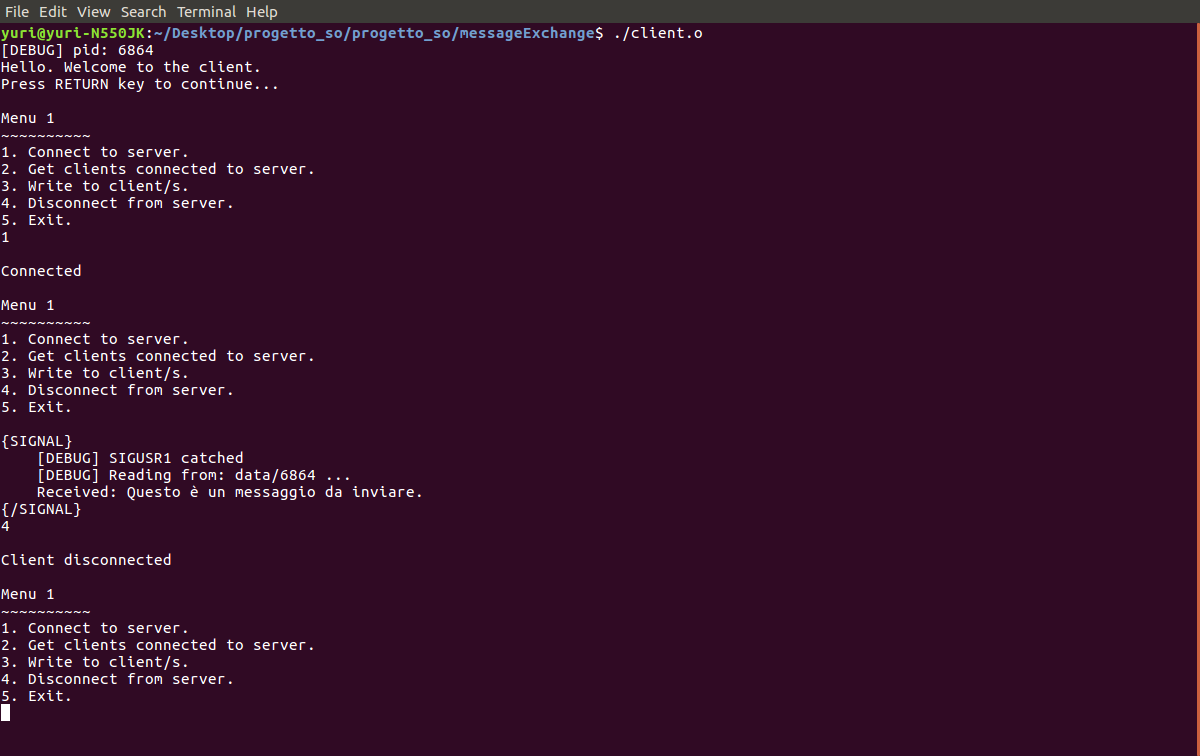
\includegraphics[width=\textwidth]{screenmsg/13_client_6864}
\caption{Disconnessione di 6864 dal server}
\end{subfigure}
\begin{subfigure}[b]{0.7\textwidth}
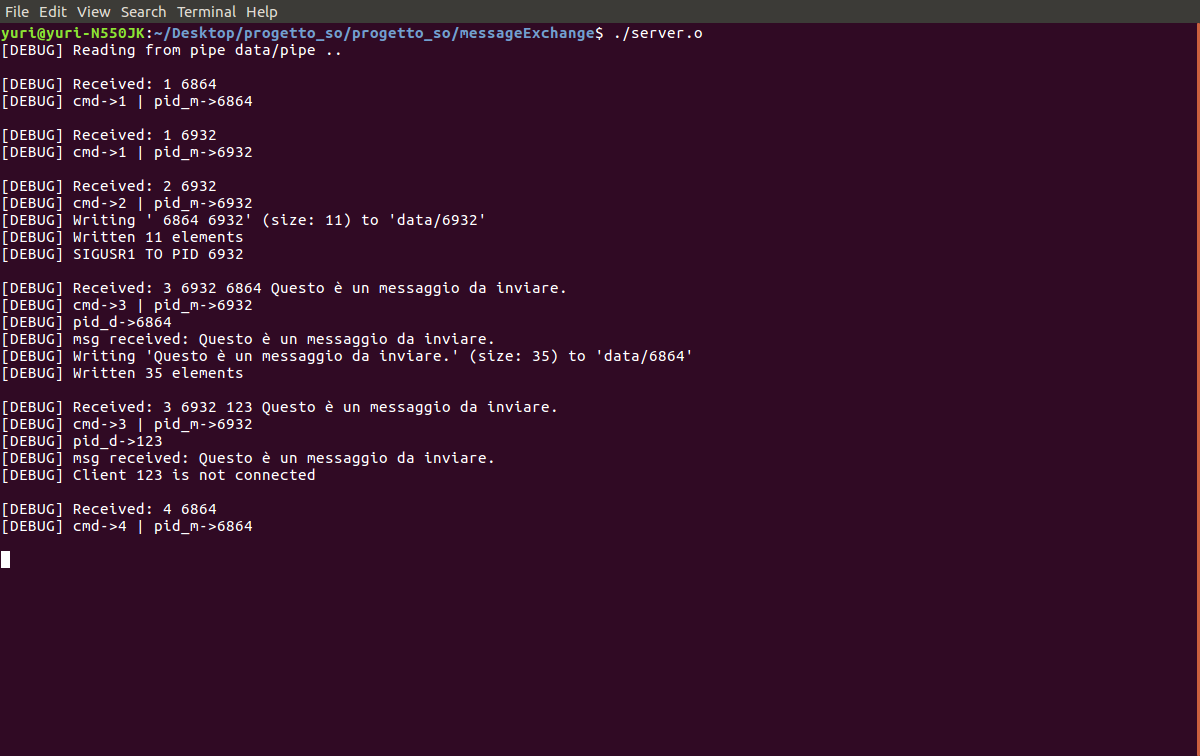
\includegraphics[width=\textwidth]{screenmsg/14_server}
\caption{Risposta del server}
\end{subfigure}
\begin{subfigure}[b]{0.7\textwidth}
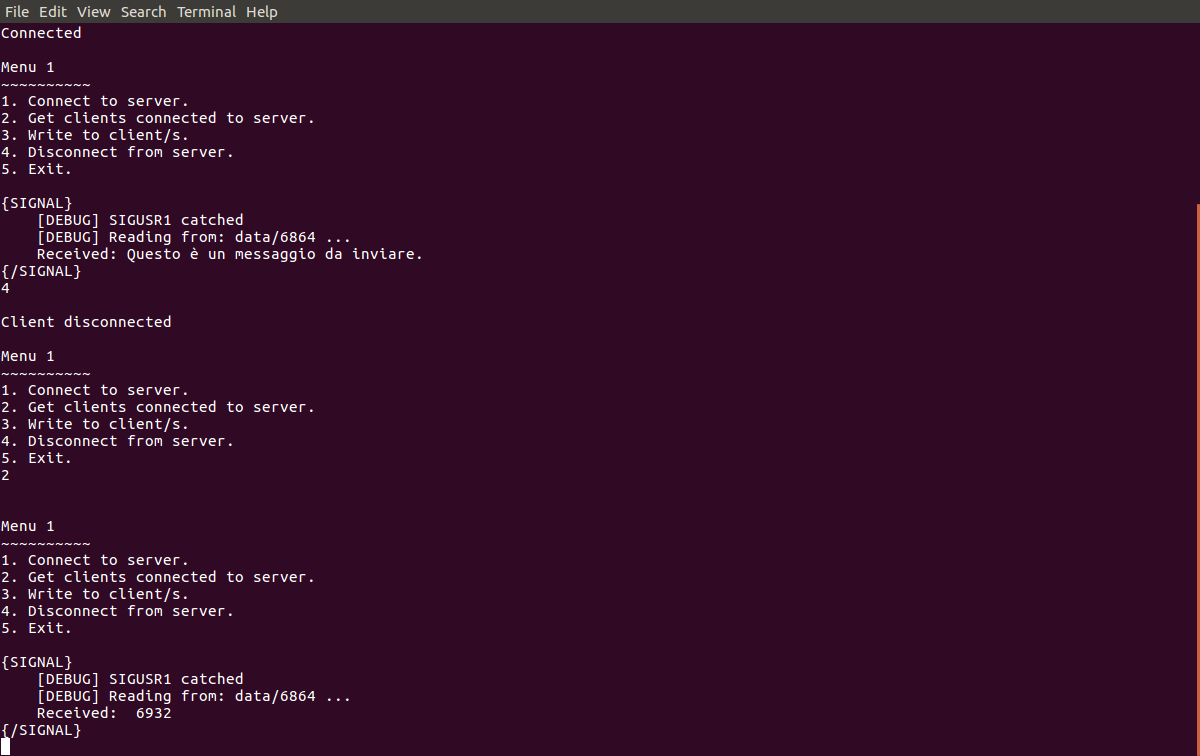
\includegraphics[width=\textwidth]{screenmsg/15_client_6864}
\caption{Richiesta dei client connessi al server}
\end{subfigure}
\caption{Disconnessione}
\end{figure}

\begin{figure}
\centering
\begin{subfigure}[b]{0.8\textwidth}
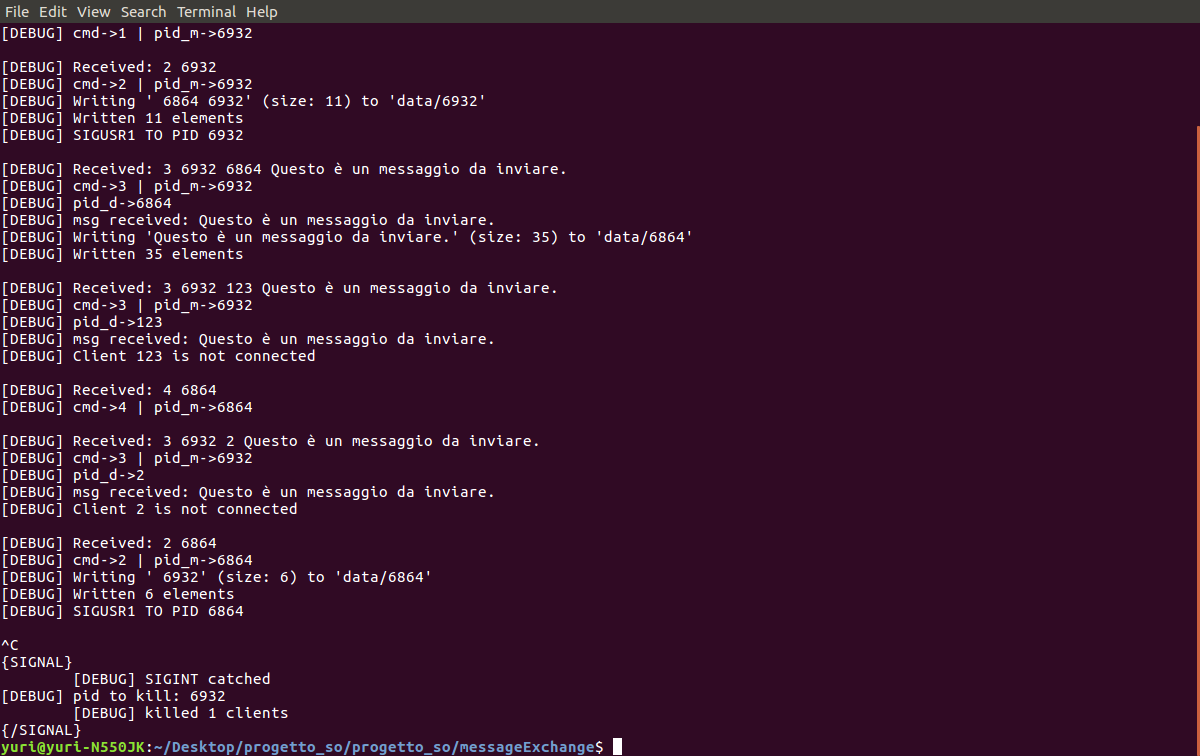
\includegraphics[width=\textwidth]{screenmsg/16_server}
\caption{}
\end{subfigure}
\begin{subfigure}[b]{0.8\textwidth}
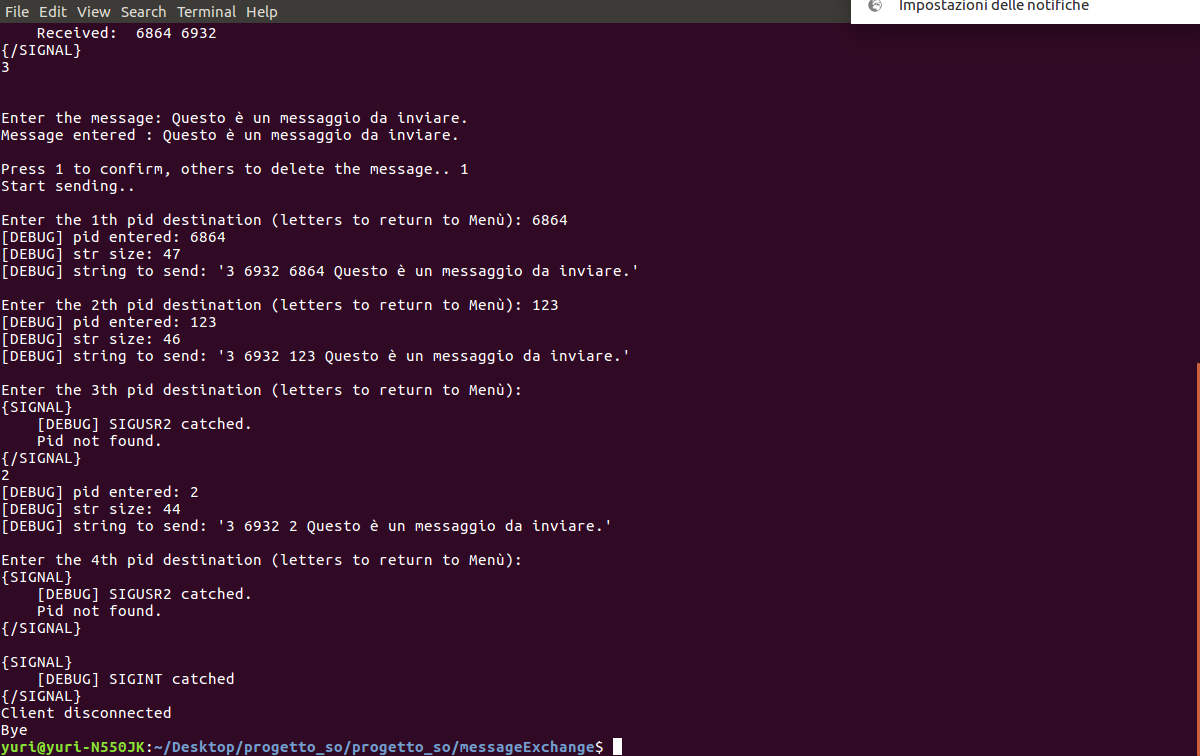
\includegraphics[width=\textwidth]{screenmsg/17_client_6932}
\caption{}
\end{subfigure}
\caption{Errori}
\end{figure}
